\documentclass[french]{beamer}
%\usepackage{listingsutf8}
%\usepackage[T1]{fontenc}
%\usepackage[utf8]{inputenc}
\usepackage{fontspec}
\usepackage[french]{babel}
\usepackage{amsmath, amssymb, mathrsfs}
\usepackage{graphicx}
\usepackage{listings}
\usepackage{tikz}
\usepackage{pgfplots}
\usepackage{epic, eepic}
\usepackage{fancybox}
\usepackage{array, multirow, tabularx}
\usepackage{algorithm,algorithmic}

\usetheme{Warsaw}
\mode<presentation>
\setbeamertemplate{navigation symbols}{}

\hypersetup{pdfpagemode=FullScreen, colorlinks=true,
  pdftitle={Présentation projet méthodes approchées.}, backref}

\title{Projet de méthodes approchées}

\institute{M1 informatique UM2}
\author{Dyce William, Loukil Amal, Ouazzani Sabrina}
\date{semestre 2 : 2011-2012}
\begin{document}

\begin{frame}
  \titlepage
\end{frame}

\section{Introduction}

\begin{frame}
  \frametitle{Problème}
  \begin{itemize}
  \item problèmes d'optimisation 
    \begin{itemize}
    \item[] $\nearrow$ problèmes faciles
    \item[] $\searrow$ \fbox{problèmes NP-difficiles}
    \end{itemize}
  \item  $\Rightarrow$ méthodes exactes 
    \begin{itemize}
    \item[] $\nearrow$ programmation dynamique
    \item[] $\searrow$ branch and bound
    \end{itemize}

    
  \item  $\Rightarrow$ méthodes approchées
    \begin{itemize}
    \item[] $\longrightarrow$ algorithmes d'approximation
    \end{itemize}
  \end{itemize}
\end{frame}

\begin{frame}
  \frametitle{Table of Contents}
  \begin{columns}
    \begin{column}[]{5cm}
      \tableofcontents
    \end{column}
    \begin{column}[]{5cm}
      \begin{center}
        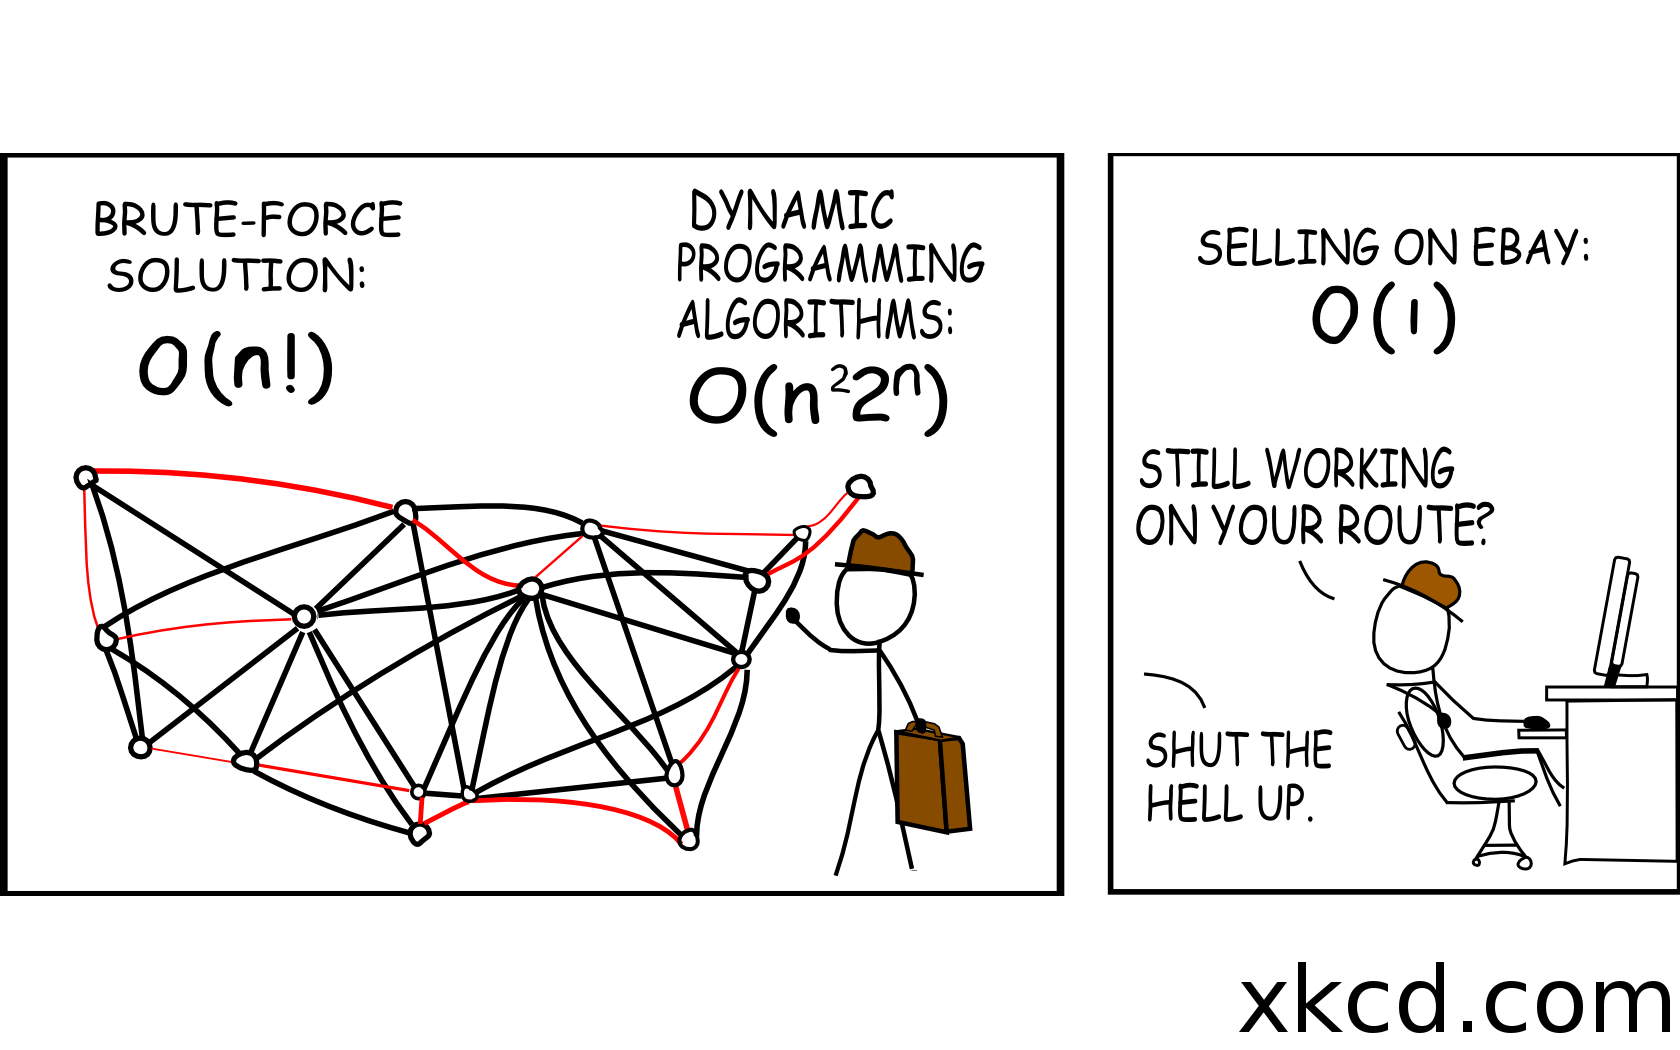
\includegraphics[height=3.5cm]{../images/commerce.png}
      \end{center}
    \end{column}
  \end{columns}
\end{frame}

\section{Programmation dynamique}

\begin{frame}
  \frametitle{Outils}
  \begin{columns}
    \begin{column}[]{5cm}
      \begin{center}
        
\includegraphics[height=3.5cm]{../images/tools.jpeg}
      \end{center}
    \end{column}
      \begin{column}[]{5cm}
         \begin{block}{Programmation}
        langage C
      \end{block}
      \begin{block}{Tests}
        \begin{itemize}
        \item tests unitaires
        \item tests de temps d'exécution
        \end{itemize}
      \end{block}
      \end{column}
    \end{columns}
  \end{frame}

\begin{frame}
  \frametitle{Partition}
  \begin{alertblock}{Formules}
    \begin{equation}
      \begin{cases}
        tab[0] = \top ; \\
	tab[j + poids[i]] = \top \text{ ssi } tab[j] ; \\
      \end{cases}
    \end{equation}
  \end{alertblock}
\begin{enumerate}
\item calcul de la somme totale 
\item retourne le booléen de la case $\dfrac{somme}{2}$
\end{enumerate}
\end{frame}

\begin{frame}
  \frametitle{Partition}
  \begin{columns}
    \begin{column}[]{4cm}
      \begin{center}
        
\includegraphics[height=3.5cm]{../images/unitest.jpg}
      \end{center}
    \end{column}
      \begin{column}[]{6cm}
        \begin{block}{Test unitaire}
	3 objets : \\
	poids : \{1, 2, 7\} \\
	réponse : $\perp$
        \end{block}
      \end{column}
    \end{columns}
\end{frame}
  \begin{frame}
  \frametitle{Partition : jeux d'essais}

\begin{table}[h!]
\centering
\begin{tabular}{|c|c|}
\hline
Nombre d'objets & temps d'exécution moyen en ms\\
\hline
150 & 1\\
\hline
500 & 14\\
\hline
650 & 24\\
\hline
800 & 32\\
\hline
950 & 43\\
\hline
1000 & 51\\
\hline
2000 & 185\\
\hline
3000 & 565\\
\hline
5000 & 1536\\
\hline
\end{tabular}
\caption {Variation du temps d'exécution en fonction du nombre d'objets}
\end{table}
\end{frame}

\begin{frame}
\frametitle{Courbe du temps d'exécution de partition}
\begin{figure}[h!]
\centering
\begin{tikzpicture}[scale=0.7]
    \begin{axis}[title=Jeux de tests pour partition, xlabel= nombre d'objets, ylabel= temps d'exécution]
      \addplot
        table[col sep=comma]{../charts/partition.csv};
        \legend{exécution de partition}
    \end{axis}
\end{tikzpicture}
\caption{Temps d'exécution de partition.}
\end{figure}

  \end{frame}
  
  
  \begin{frame}
    \frametitle{Sac à dos}
    \begin{alertblock}{Formules}
      \begin{equation}
        \begin{cases}
          tab[0][w] = 
          \begin{cases} 
            \text{0 si } w < poids[0] \\
            utilite[0] \text{ sinon} \\
          \end{cases} \\

          tab[i][j] = max(tab[i-1] [j], (tab[i-1] [j-poids[i]] + utilite[i])); \\
        \end{cases}
      \end{equation}
    \end{alertblock}
  \end{frame}

\begin{frame}
  \frametitle{Sac à dos}
  \begin{columns}
    \begin{column}[]{3cm}
      \begin{center}
        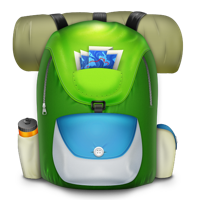
\includegraphics[height=3cm]{../images/Knapsack.png}
      \end{center}
    \end{column}
      \begin{column}[]{7cm}
        \begin{block}{Test unitaire}
		7 objets : \\
		capacité : 2\\
		poids : \{3, 5, 1, 5, 7, 2, 6\} \\
		utilités : \{2, 5, 3, 3, 6, 2, 4\} \\
		réponse : 3 \\
        \end{block}
      \end{column}
    \end{columns}
  \end{frame}


  \begin{frame}
    \frametitle{Sac à dos : variation du nombre d'objets}
\begin{table}[h!]
\centering
\begin{tabular}{|c|c|}
\hline
Nombre d'objets & temps d'exécution moyen en ms\\
\hline
100 & 8\\
\hline
150 & 12\\
\hline
200 & 16\\
\hline
300 & 24\\
\hline
500 & 40\\
\hline
800 & 65\\
\hline
1000 & 82\\
\hline
1200 & 101\\
\hline
2000 & 165\\
\hline
3000 & 246\\
\hline
 4000 & 329\\
\hline
  5000 & 410\\
\hline
\end{tabular}
\caption {Variation du temps d'exécution en fonction du nombre d'objets}
\end{table}
  \end{frame}

  \begin{frame}
    \frametitle{Courbe variation du nombre d'objets}
\begin{figure}[h!]
\centering
\begin{tikzpicture}[scale=0.7]
    \begin{axis}[title=Jeux de tests pour Sac à dos, xlabel= nombre d'objets, ylabel= temps d'exécution]
      \addplot
        table[col sep=comma]{../charts/sac.csv};
        \legend{exécution de sac à dos}
    \end{axis}
\end{tikzpicture}
\caption{Temps d'exécution de sac à dos.}
\end{figure}
  \end{frame}

 \begin{frame}
    \frametitle{Sac à dos : variation de la capacité maximale du sac}
\begin{table}[h!]
\centering
\begin{tabular}{|c|c|}
\hline
Capacité & temps d'exécution moyen en ms\\
\hline
500 & 0\\
\hline
1000 & 1\\
\hline
2000 & 3\\
\hline
2500 & 3\\
\hline
3000 & 4\\
\hline
4000 & 6\\
\hline
5000 & 8\\
\hline
10000 & 16\\
\hline
\end{tabular}
\caption {Variation du temps d'exécution en fonction du capacité du sac}
\end{table}
  \end{frame}

  \begin{frame}
    \frametitle{Courbe variation de la capacité maximale du sac}
\begin{figure}[h!]
\centering
\begin{tikzpicture}[scale=0.7]
    \begin{axis}[title=Jeux de tests pour Sac à dos, xlabel= capacité, ylabel= temps d'exécution]
      \addplot
        table[col sep=comma]{../charts/sac1.csv};
        \legend{exécution de sac à dos}
    \end{axis}
\end{tikzpicture}
\caption{Temps d'exécution de sac à dos.}
\end{figure}
  \end{frame}

  \begin{frame}
    \frametitle{Voyageur de commerce}
    \begin{alertblock}{Formules}
      \begin{equation}
        \begin{cases}
          C[\{0\}][i] = poids[0][i] \\
          C[S][i] = min_{k \in S - \{ 0 \}} \{ C[S- \{ k \}][k] + poids[k][i]  \}
        \end{cases} 
      \end{equation}
      \begin{equation}
      	opt = min_{i}C[\{0, 1, \dots, n\} - \{ i\}, i] + poids[i][0]
      \end{equation}
    \end{alertblock}
  \end{frame}

\begin{frame}
  \frametitle{Voyageur de commerce}
  \begin{columns}
    \begin{column}[]{5cm}
      \begin{center}
        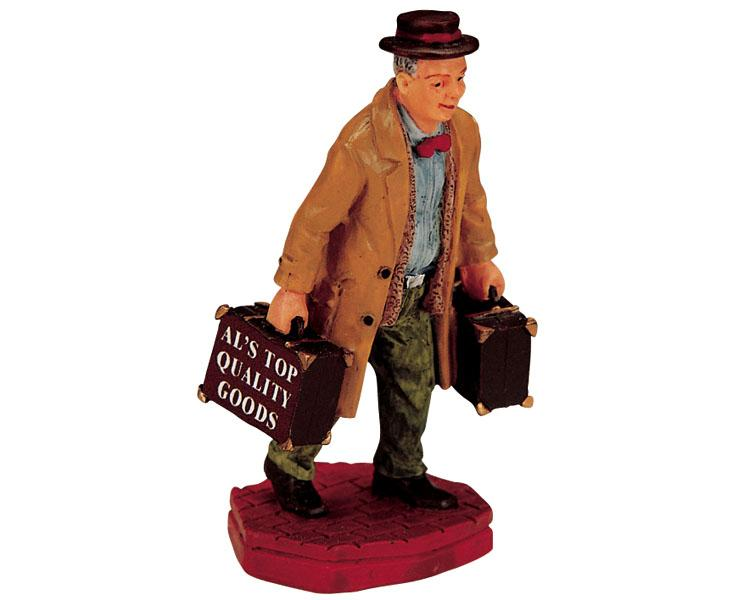
\includegraphics[height=4cm]{../images/salesman2.jpg}
      \end{center}
    \end{column}
      \begin{column}[]{6cm}
        \begin{block}{Test unitaire}
	5 villes : \\
	distances 1 : \{0, 1, 2, 1, 0\} \\
	distances 2 : \{1, 0, 3, 5, 0\} \\
	distances 3 : \{2, 3, 0, 2, 1\} \\
	distances 4 : \{1, 5, 2, 0, 4\} \\
	distances 5 : \{0, 0, 1, 4, 0\} \\
	réponse : 5
        \end{block}
      \end{column}
    \end{columns}
  \end{frame}

\begin{frame}
\frametitle{Voyageur de commerce : jeux d'essai}
\begin{table}[h!]
\centering
\begin{tabular}{|c|c|}
\hline
Sommets & temps d'exécution moyen en ms\\
\hline
2 & 0\\
\hline
5 & 2\\
\hline
7 & 15\\
\hline
9 & 137\\
\hline
11 & 1151\\
\hline
13 & 8575\\
\hline
15 & 58109\\
\hline
\end{tabular}
\caption {Variation du temps d'exécution en fonction du capacité du sac}
\end{table}
\end{frame}

\begin{frame}
\frametitle{Voyageur de commerce : courbe}
\begin{figure}[h!]
\centering
\begin{tikzpicture}[scale=0.7]
    \begin{axis}[title=Jeux de tests pour le TSP, xlabel= nombre de
        villes parcourues, ylabel= temps d'exécution]
      \addplot
        table[col sep=comma]{../charts/tspdyn.csv};
        \legend{exécution de sac à dos}
    \end{axis}
\end{tikzpicture}
\caption{Temps d'exécution du voyageur de commerce.}
\end{figure}
\end{frame}

\section{Branch and Bound TSP}

\begin{frame}
  \frametitle{Branch and Bound TSP}
  \begin{block}{Outils}
Ocaml
  \end{block}
\end{frame}

\begin{frame}
\frametitle{Principe du branch and bound TSP}
\begin{enumerate}
 \item faire ACPM $G - \{x \}$
  \item relier $x$ à ses deux voisins les plus proches en terme de coût
  \item si {valeur du cycle > borne inférieure}
   \begin{itemize}
\item si {tous les sommets sont de degré $2$} alors mettre à jour le solution courante
\item sinon, choisir un sommet $y$ de degré $\geq$ 2
\begin{itemize}
\item  pour {chaque arête $e_i$ issue de $y$}
\item  $G' := G - \{ e_i \}$
\item BranchAndBound($y$, borne inférieure, $G'$)
\end{itemize}
\end{itemize}
    \item retourner la plus petite des solutions acceptables
\end{enumerate}

\end{frame}

\begin{frame}
  \frametitle{Solution initiale}
  \begin{itemize}
  \item chaîne de poids le plus faible~;
  \item voisinage 2--opt~;
  \item voisinage 3--opt.
  \end{itemize}
\end{frame}

\section{Algorithme $\frac{3}{2}$ TSP}

\begin{frame}
\frametitle{$\frac{3}{2}$ approximation TSP}
\begin{block}{Outils}
  \begin{itemize}
  \item langage C/C++
  \item bibliothèque Boost Graph
  \item gprof
  \end{itemize}
\end{block}
\end{frame}

\begin{frame}
\frametitle{Principe du $\frac{3}{2}$ approximation TSP}
\begin{enumerate}
\item faire ACPM $T$ $G$ de coût $w$
\item $W := $ sommets de degré impair de $T$
\item chercher un couplage $M$ de $G$ poids min $m$ saturant tous les
sommets de $W$
\item $G' := $ le graphe construit à partir des arêtes de $M$ et de
$T$
\item Soit P un parcours eulérien de longueur $p$, on a $p:= w + m$
\item retourner un cycle de longueur $c \leq p$
\end{enumerate}
\end{frame}

\section{Conclusion}
\begin{frame}
\begin{itemize}
\item programmation dynamique
\item structure de données
\item algorithmes de TSP
\end{itemize}
\end{frame}


\begin{frame}
  \begin{center}
    Merci pour votre attention.
  \end{center}
\end{frame}

\end{document}
